\documentclass[12pt,a4paper]{article}
\topmargin -1.6cm
\addtolength{\textheight}{4cm}
\textwidth  15.5cm

\leftmargin      5mm
\rightmargin     5mm
\oddsidemargin   5mm
\evensidemargin  5mm

\usepackage{hyperref}
\usepackage{polski}
\usepackage[utf8]{inputenc}
\usepackage{graphicx}
\usepackage{units}
\usepackage{sty/style}
\usepackage{float}

\projekt{Modelowanie obiektu manipulatora 2R (EDDA)}
\autor{Marcin Bober, 249426}
\przedmiot{Projekt specjalnościowy ARR}
\prowadzacy{Dr inż. Mirela Kaczmarek}

\begin{document}
\pdfpageheight   297mm
\pdfpagewidth    210mm

\StronaTytulowa
\SpisTresci

\pagebreak

\section{Cel ćwiczenia}
  Celem ćwiczenia jest zbadanie zachowania dwóch algorytmów sterowania sprzężonych z manipulatorem 2R. Mają one zrealizować zadanie śledzenia zadanej trajektorii.

\section{Algorytm Qui Dorsey'a}
  \subsection{Opis} %(algorytmu i obiektu)
    Algorytm Qui Dorsey'a jest algorytmem globalnym. Jego zasada działania jest tożsama z działaniem liniowego regulatora PD. Z powodu liniowej natury algorytmu i nieliniowego charakteru obiektu, sterowanie obiektem nie będzie proste. W celu zbadania właściwości nastaw regulatora na błąd śledzenia trajektorii (uchyb) został przeprowadzony szereg symulacji. Przetestowane nastawy wraz z rzędem błędu sterowania zostały podane w tabeli \ref{table:1}.

  \subsection{Wyniki} %tabelka - zmiany nastaw a rząd błędu
    W tabeli \ref{table:1} znajduje się zestaw sześciu par nastaw dla KP i KD regulatora. W kolejnych kolumnach został umieszczony rząd błędu sterowania odpowiadający podany parametrom. 

  \begin{table}[h!]
    \centering
    \begin{tabular}{ r | r | c | c }
      P & D & $e_1$ & $e_2$  \\ 
      \hline
      10 & 1 & $10^{-1}$ & $10^{-1}$ \\  
      100 & 10 & $10^{-1}$ & $10^{-2}$ \\  
      1000 & 100 & $10^{-2}$ & $10^{-3}$ \\  
      10000 & 1000 & $10^{-3}$ & $10^{-4}$ \\  
      100000 & 10000 & $10^{-4}$ & $10^{-5}$ \\  
      1000000 & 100000 & $10^{-5}$ & $10^{-6}$ \\
      10000000 & 1000000 & $10^{-6}$ & $10^{-7}$
    \end{tabular}
    \caption{Nastawy PD i odpowiadający im rząd błędu}
    \label{table:1}
  \end{table}

    Dziesięciokrotny wzrost wzmocnienia skutkuje dziesięciokrotnym spadkiem błędu. Błędy drugiego przegubu są niższe niż dla pierwszego. Dla nastaw dążących do nieskończoności, błąd śledzenia zmierza do zera.

  \begin{figure}[H]
    \centering
    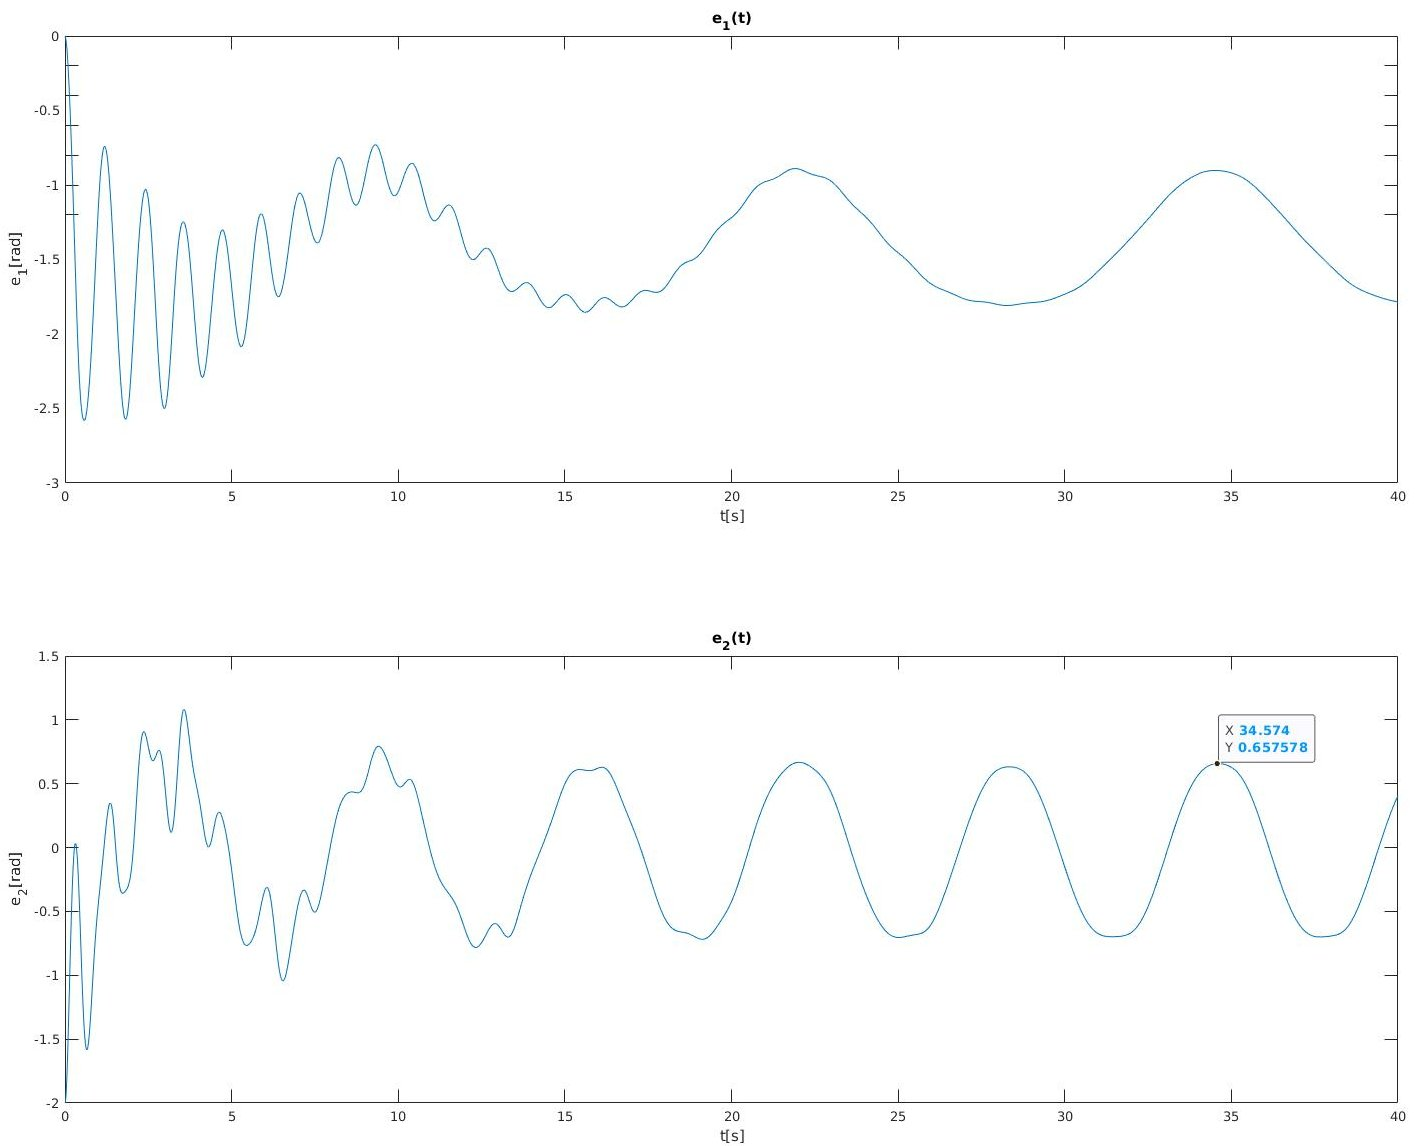
\includegraphics[height=0.4\textheight]{figures/qui10.jpg}
    \caption{KP = 10, KD = 1}
    \label{fig:10}
  \end{figure}

    Niewielkie nastawy sprawiają że obiekt ma znaczne problemy ze śledzeniem zadanej trajektorii. Błąd śledzenia dla  KP = 10 i KD = 1 w zależności do czasu został zaprezentowany na rysunku \ref{fig:10}.

  \begin{figure}[H]
    \centering
    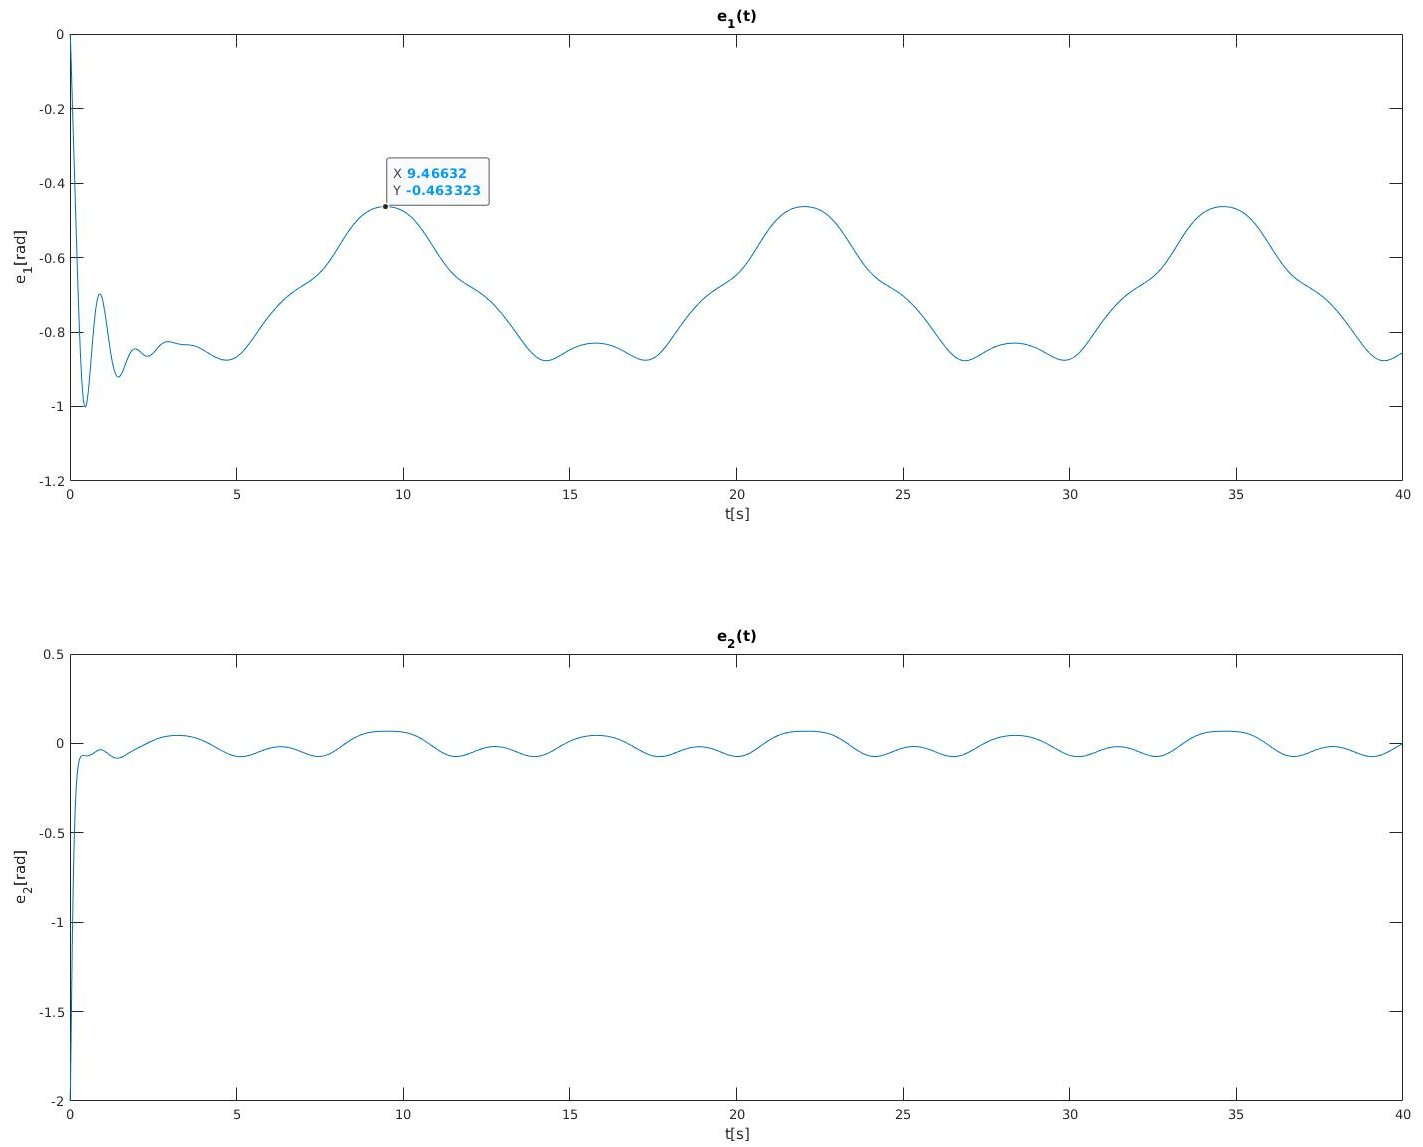
\includegraphics[height=0.4\textheight]{figures/qui100.jpg}
    \caption{KP = 100, KD = 10}
    \label{fig:100}
  \end{figure}

    Konsekwentne zwiększanie nastaw regulatora przynosi wymierne efekty w postaci malejącego błędu. Można je zaobserwować porównująć wykresy \ref{fig:1000} oraz \ref{fig:10000}.

  \begin{figure}[H]
    \centering
    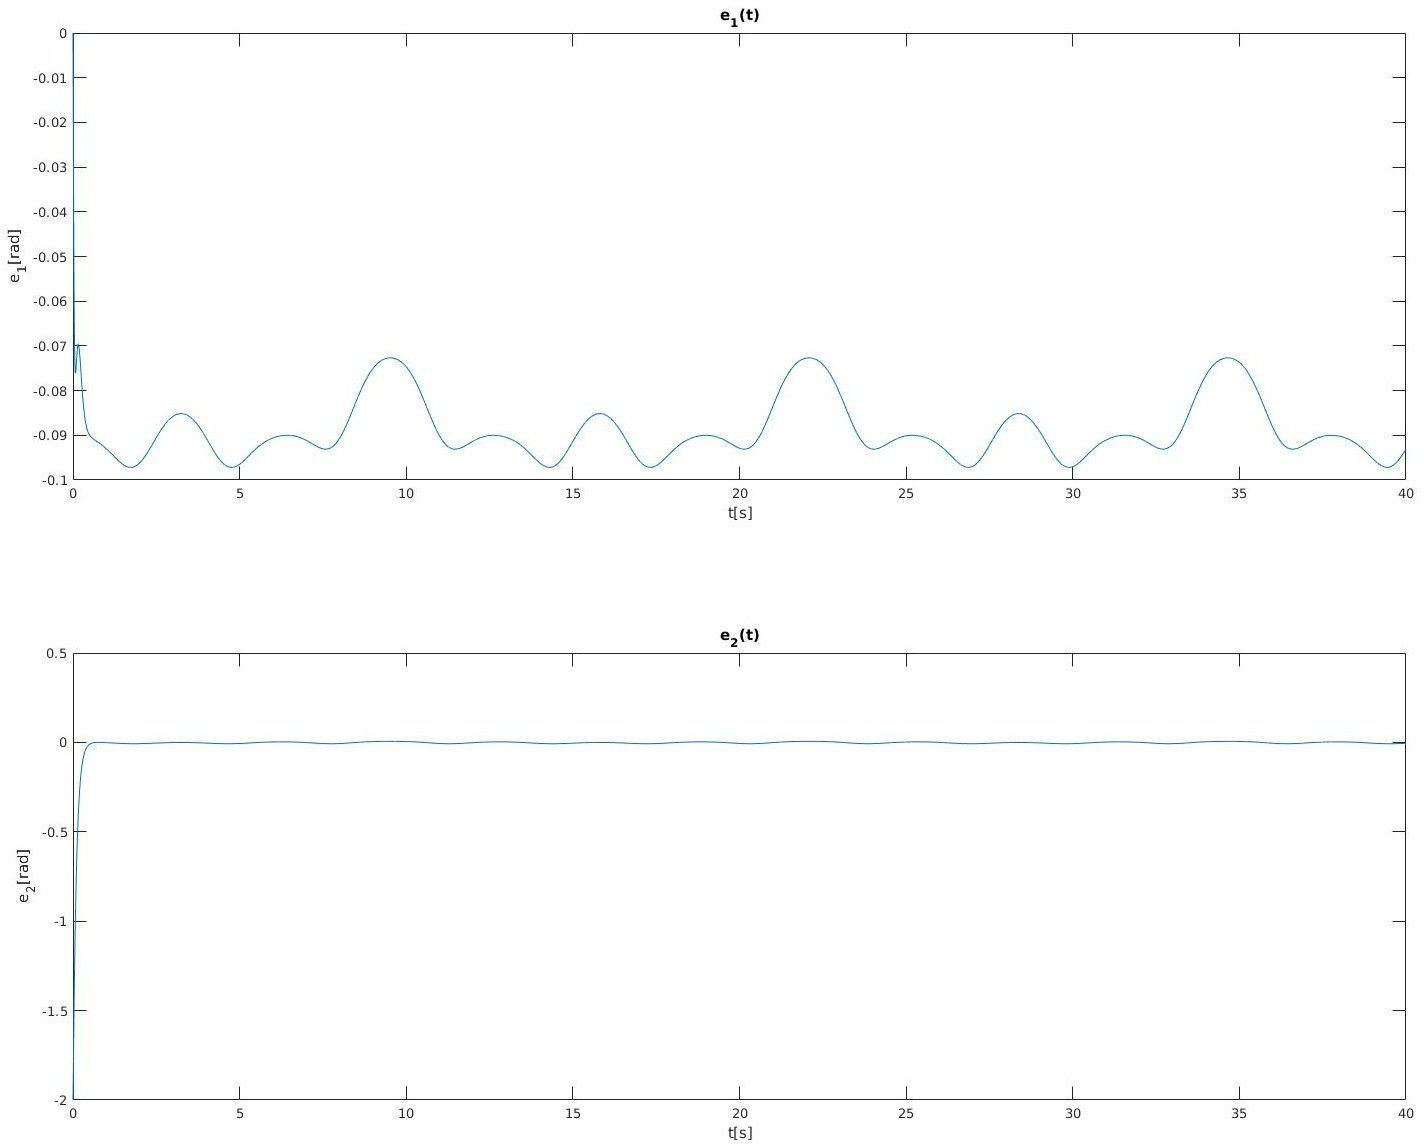
\includegraphics[height=0.4\textheight]{figures/qui1000.jpg}
    \caption{KP = 1000, KD = 100}
    \label{fig:1000}
  \end{figure}


  \begin{figure}[H]
    \centering
    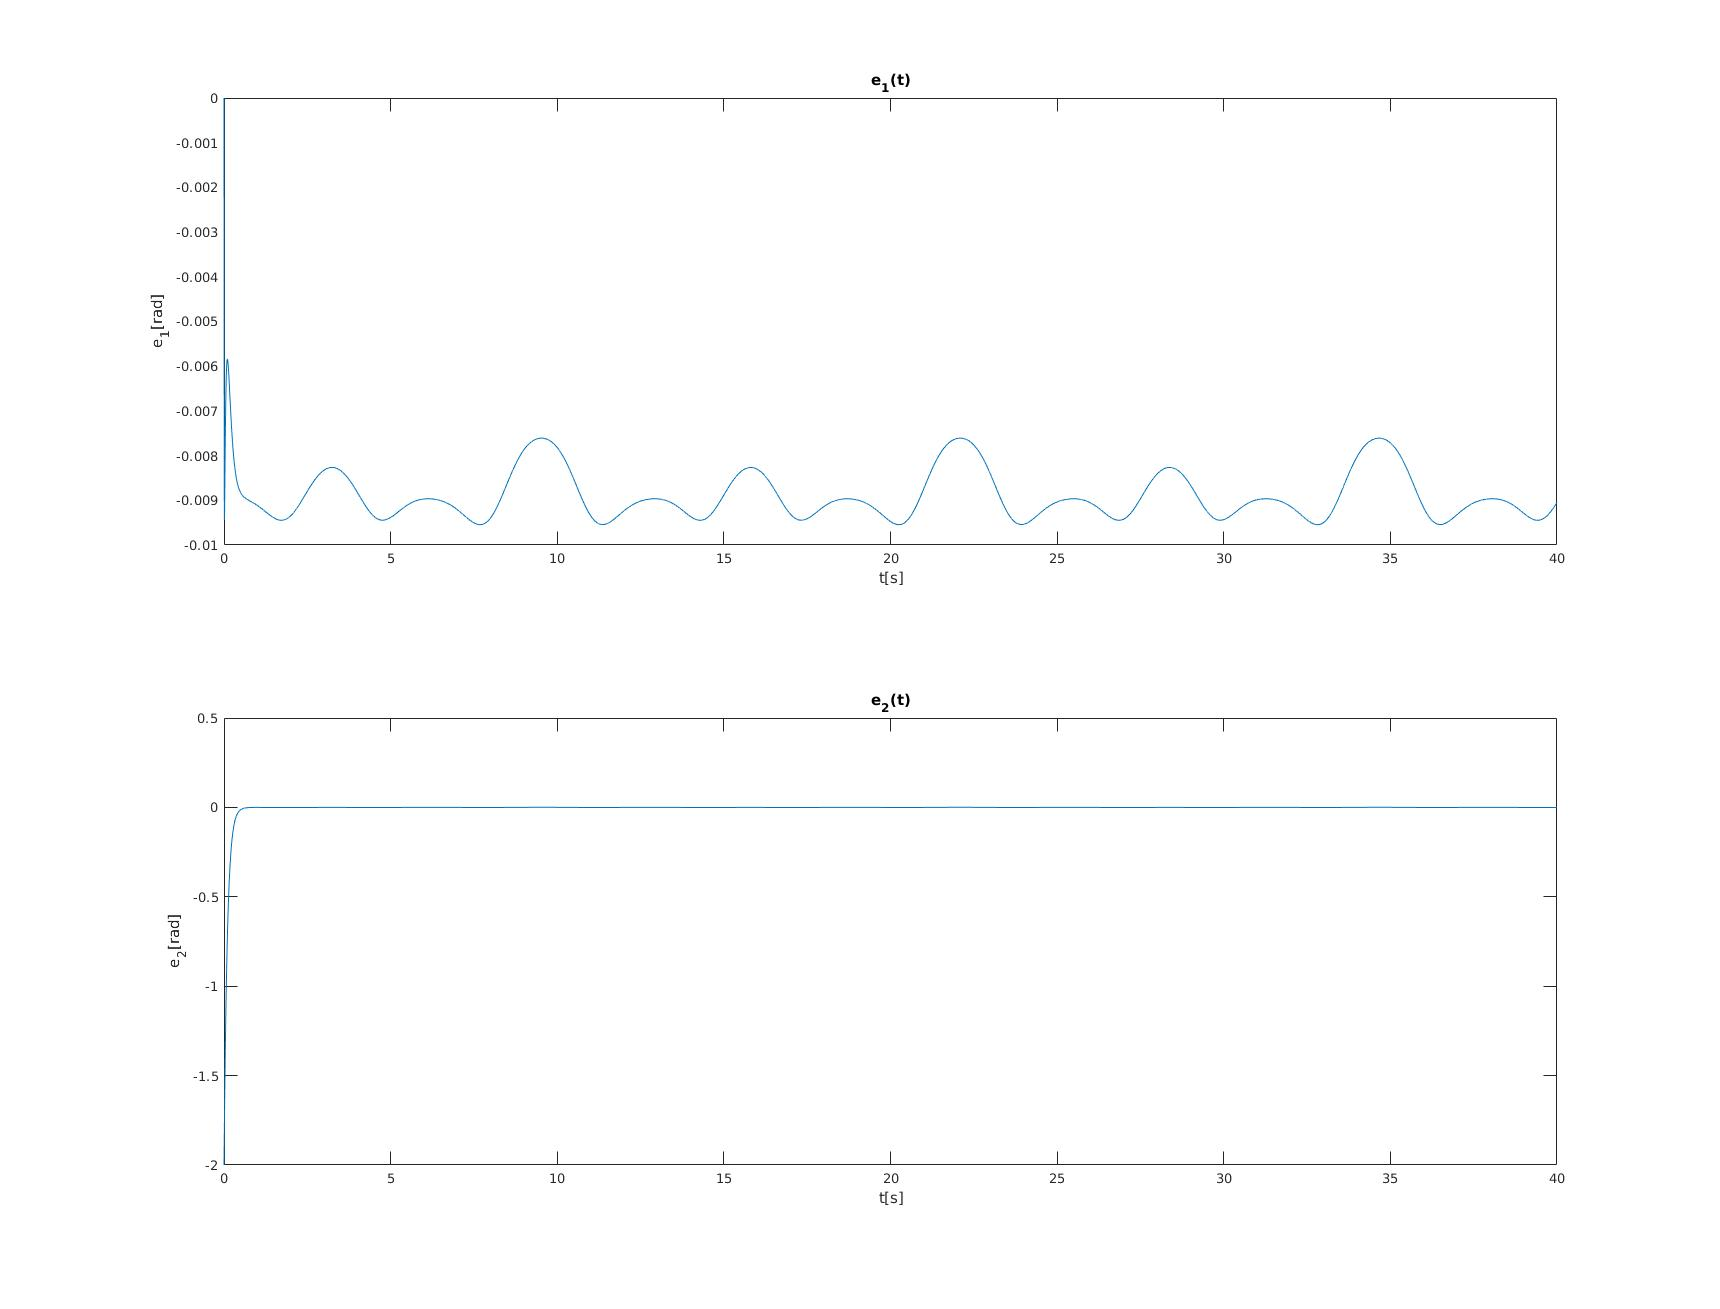
\includegraphics[height=0.4\textheight]{figures/qui10000.jpg}
    \caption{KP = 10000, KD = 1000}
    \label{fig:10000}
  \end{figure}

    Pomimo malejącego błedu należy zaznaczyć że uzyskane przbiegi w każdej iteracji posiadają charakter niegasnących oscylacji. 

  \begin{figure}[H]
    \centering
    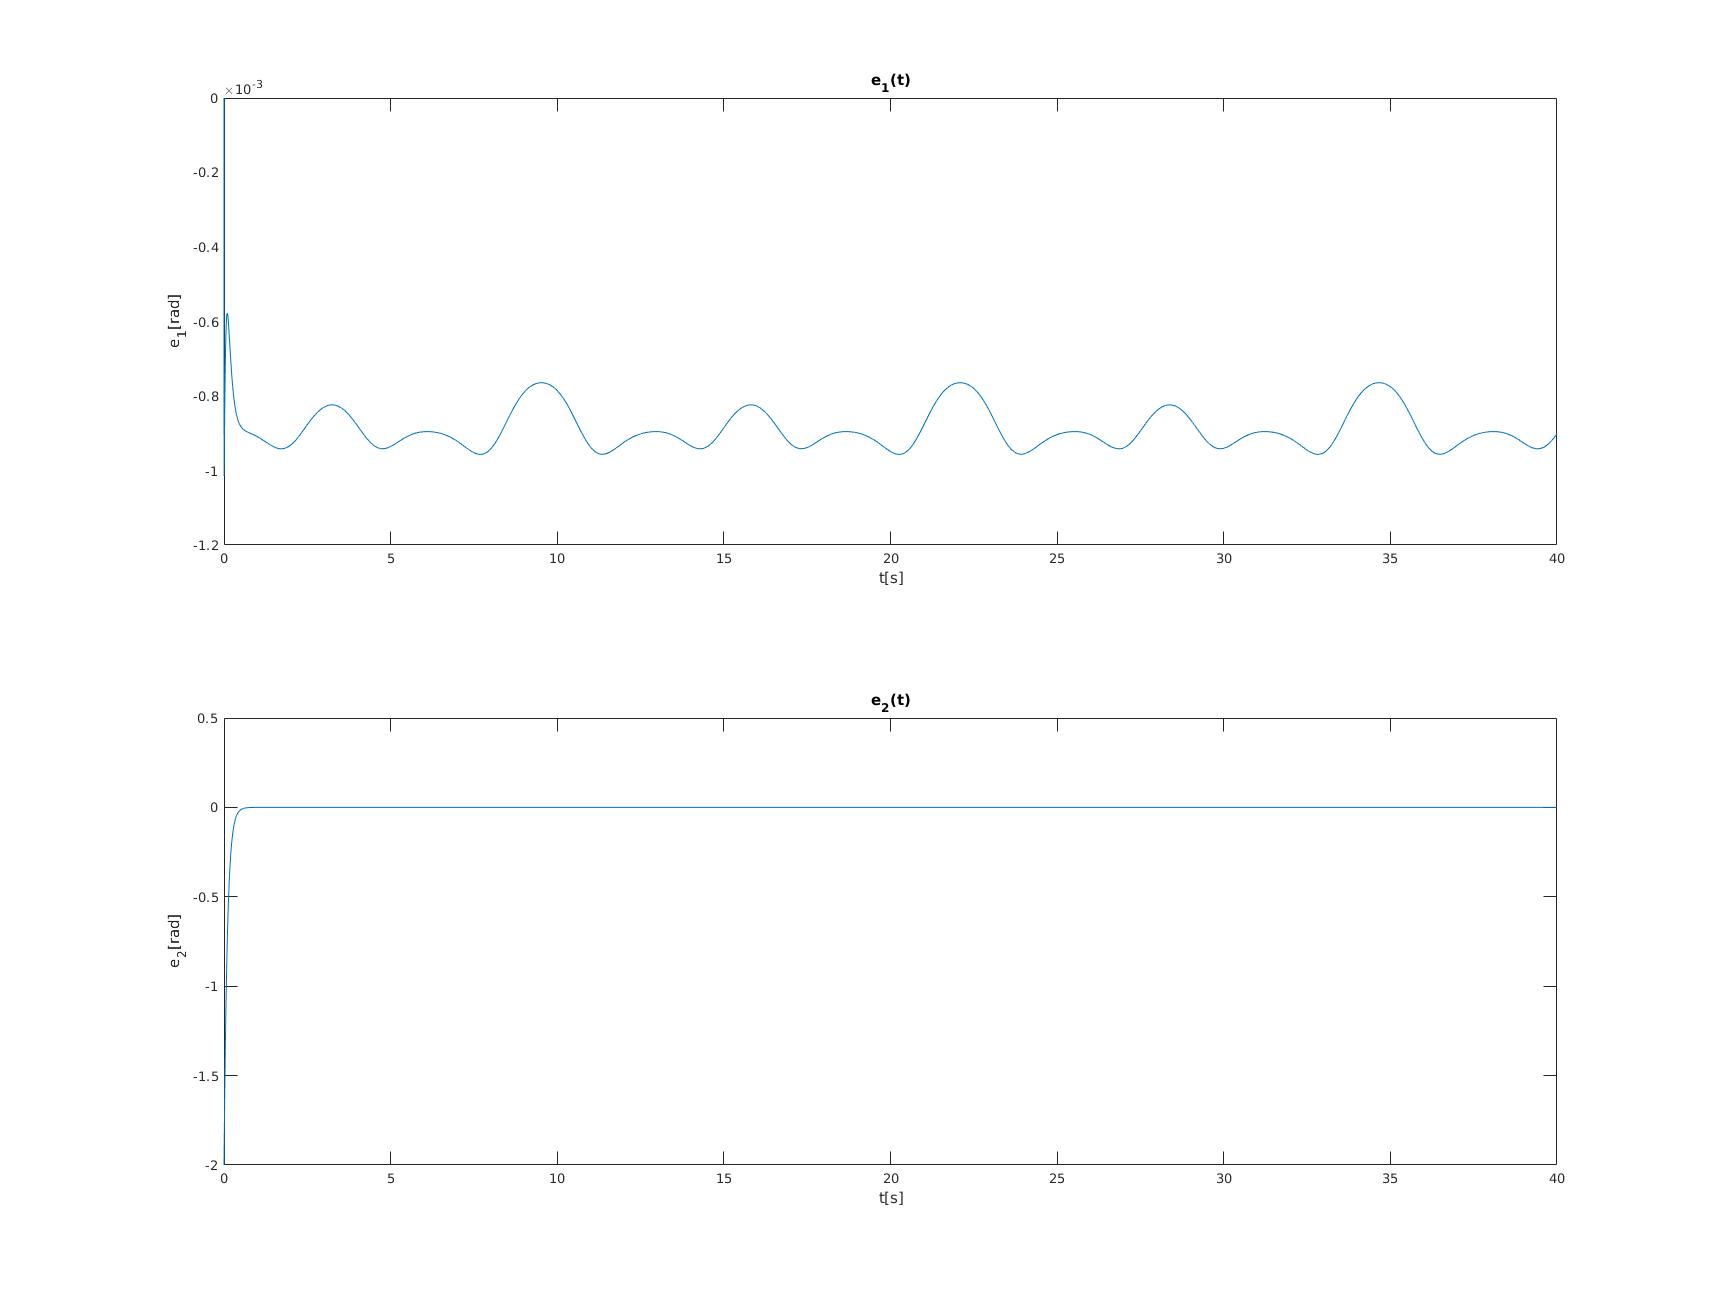
\includegraphics[height=0.38\textheight]{figures/qui100000.jpg}
    \caption{KP = 100000, KD = 10000}
    \label{fig:100000}
  \end{figure}

  \begin{figure}[H]
    \centering
    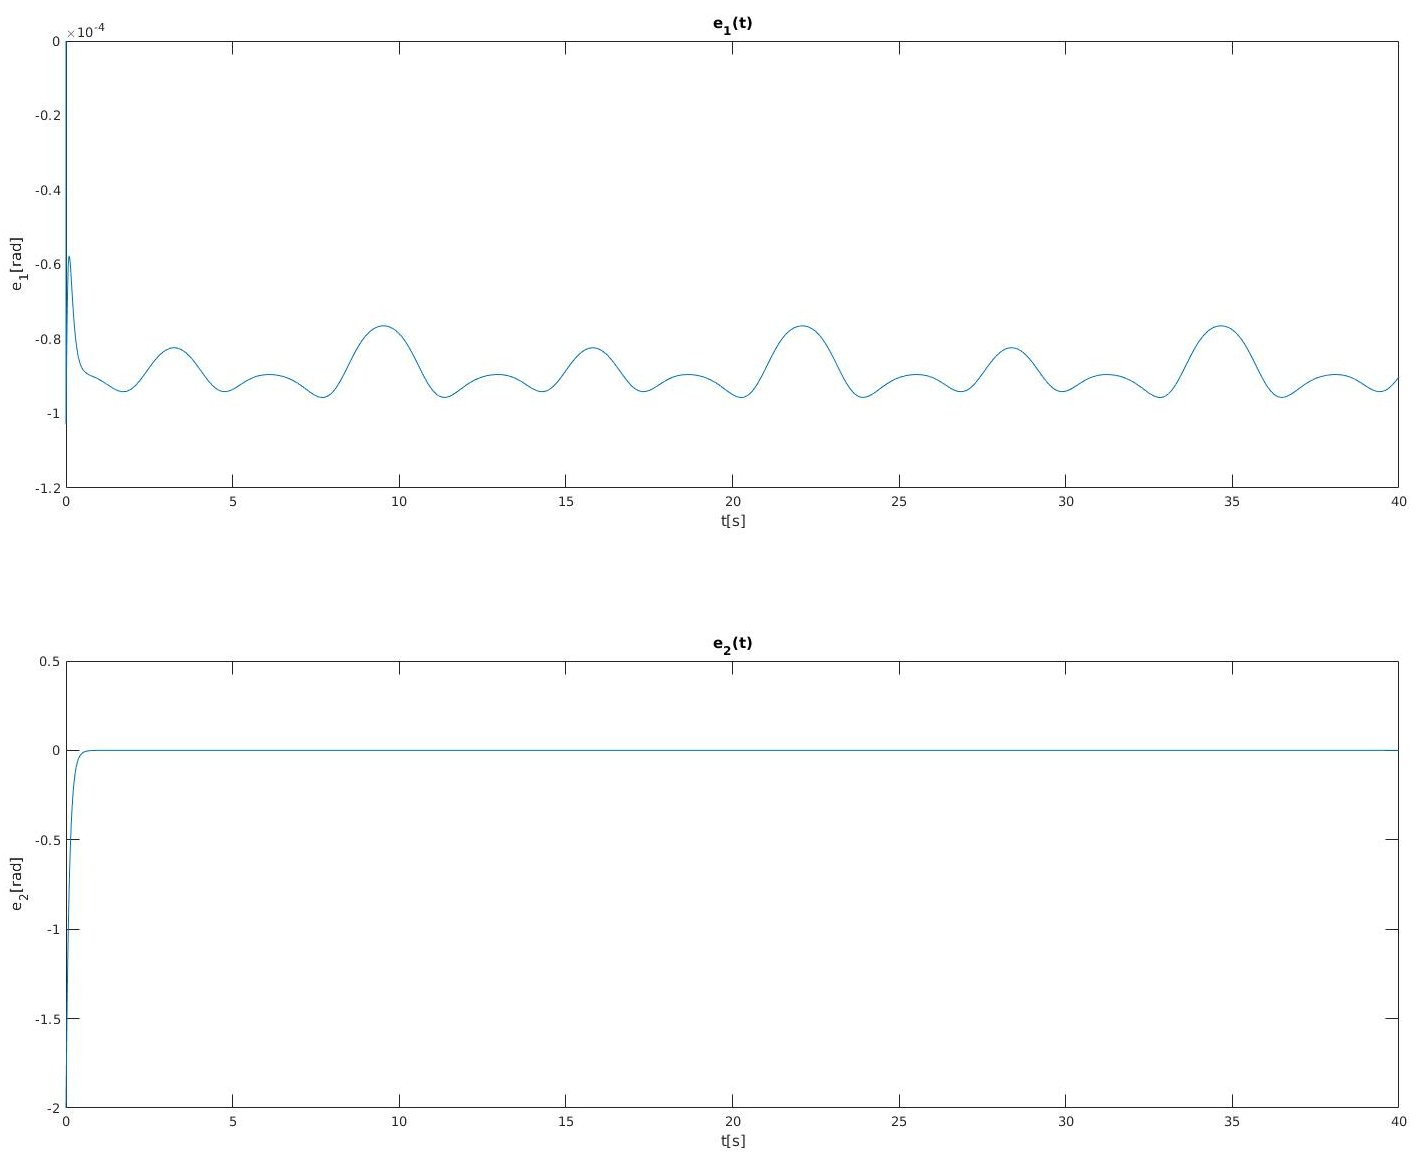
\includegraphics[height=0.38\textheight]{figures/qui1000000.jpg}
    \caption{KP = 1000000, KD = 100000}
    \label{fig:1000000}
  \end{figure}

    Stosowanie coraz to większych parametrów regulatora PD powoduje znaczący wzrost złożoności obliczeniowej.

  \subsection{Wnioski}
    Symulacje wykazały że algorytm realizuje cel minimalizacji błędu śledzenia dokładnej w przypadku zastosowania większych nastaw. Jednakże osiągnięcie zerowego błędu nie jest możliwe ponieważ wymagałoby ono nieskończonej wartości nastaw. W każdym zbadanym przypadku przebiegi błędów mają charakter niegasnących oscylacji.


\section{Algorytm dokładnej linearyzacji}
  \subsection{Opis} %(algorytmu i obiektu)
    Algorym dokładnej linearyzacji może być zastosowany jedynie dla obiektów z pełni znanych. Pierwszym etapem jest przeprowadzenie linearyzacji statycznej w celu otrzymania układu liniowego podówjego integratora.
  \subsection{Zależność od nastaw KP}
    Symulacje przeprowadzono przy stałym wzmocnieniu KD wynoszącym 1 oraz zmianie parametru KP według tabeli \ref{table:2}.

    \begin{figure}[H]
      \centering
      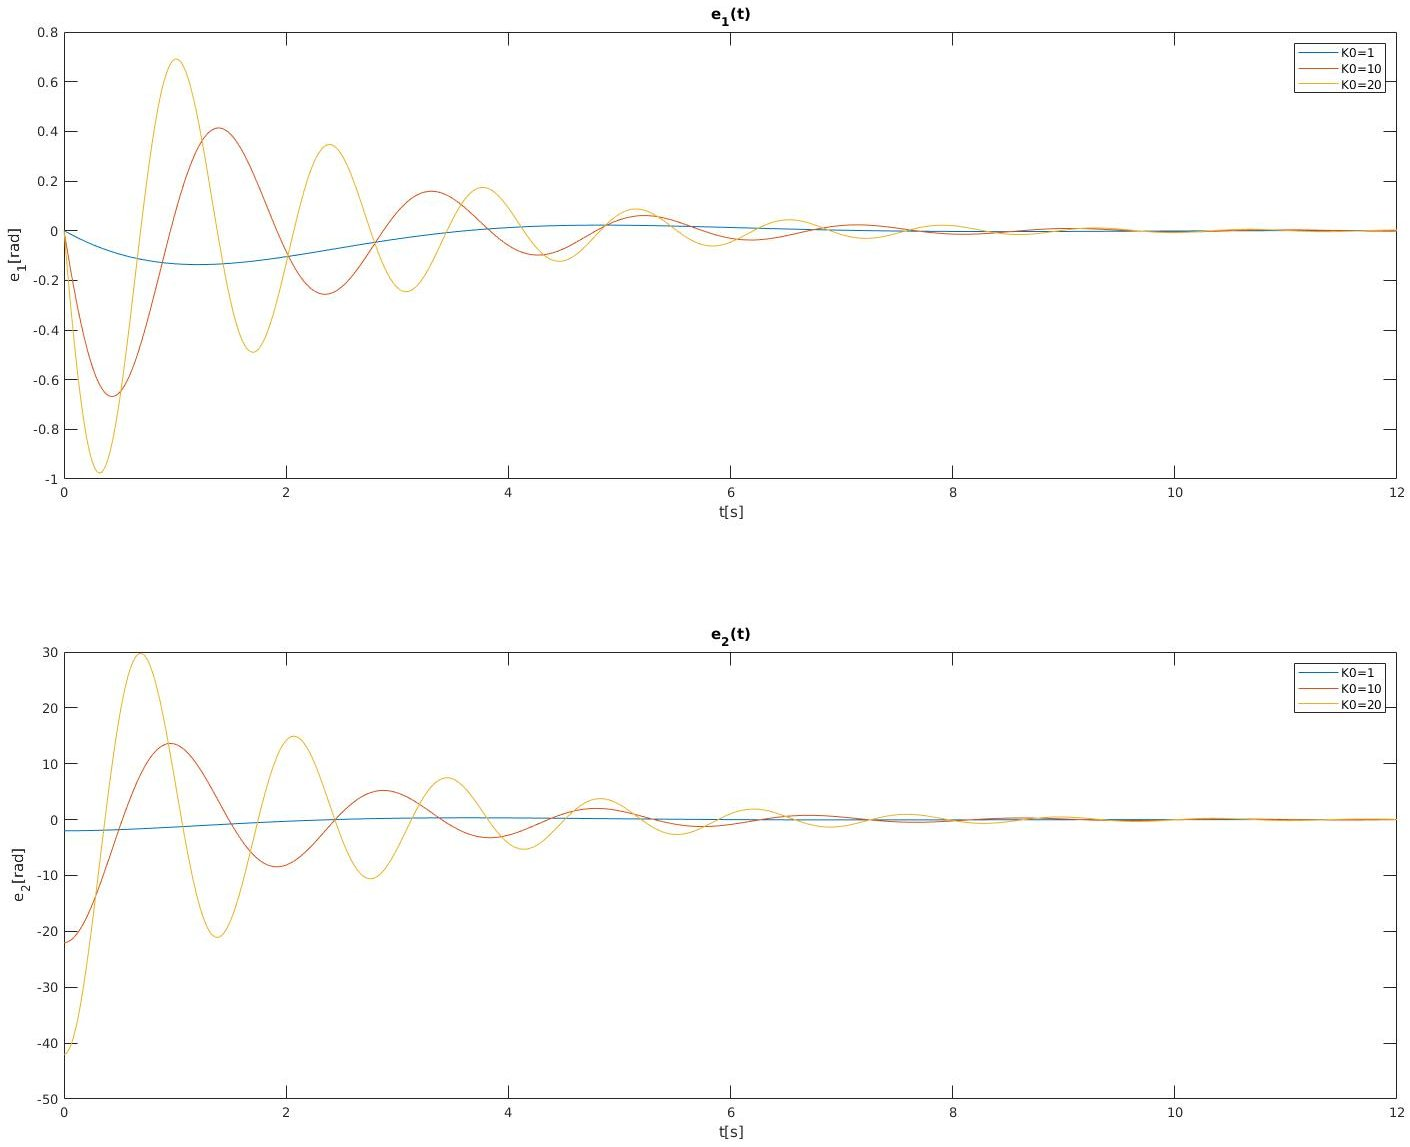
\includegraphics[height=0.50\textheight]{figures/lin1.jpg}
      \caption{stałe KD = 1, zmienne KP}
      \label{fig:lin1}
    \end{figure}

    \begin{table}[h!]
      \centering
      \begin{tabular}{ r | c | c }
        KP & Przesterowanie $e_1$ [rad] & Przesterowanie $e_2$ [rad] \\ 
        \hline
        1 & 0.16 & 0.33  \\
        10 & 1.08 & 21.36   \\
        20 & 1.66 & 49.91
      \end{tabular}
      \caption{Przesterowanie przebiegów w zależności od KP}
      \label{table:2}

      \begin{tabular}{ r | c | c }
        KP & Czas wygaszania $e_1$ [s] & Czas wygaszania $e_2$ [s]  \\ 
        \hline
        1  &  8 & 7 \\
        10 & 15 & 13  \\
        20 & 20 & 15
      \end{tabular}
      \caption{Czas wygaszania prebiegów w zależności od KP}
      \label{table:3}

    \end{table}

    Na wykresach \ref{fig:lin1} zaobserwowano znaczny wzrost przesterowania oraz czasu wygaszania wraz ze wzrostem wzmocnienia KP.

  \subsection{Zależność od nastaw KD}
  Symulacje przeprowadzono przy stałym wzmocnieniu KP wynoszącym 1 oraz zmianie parametru KD według tabeli \ref{table:3}.

  \begin{figure}[H]
    \centering
    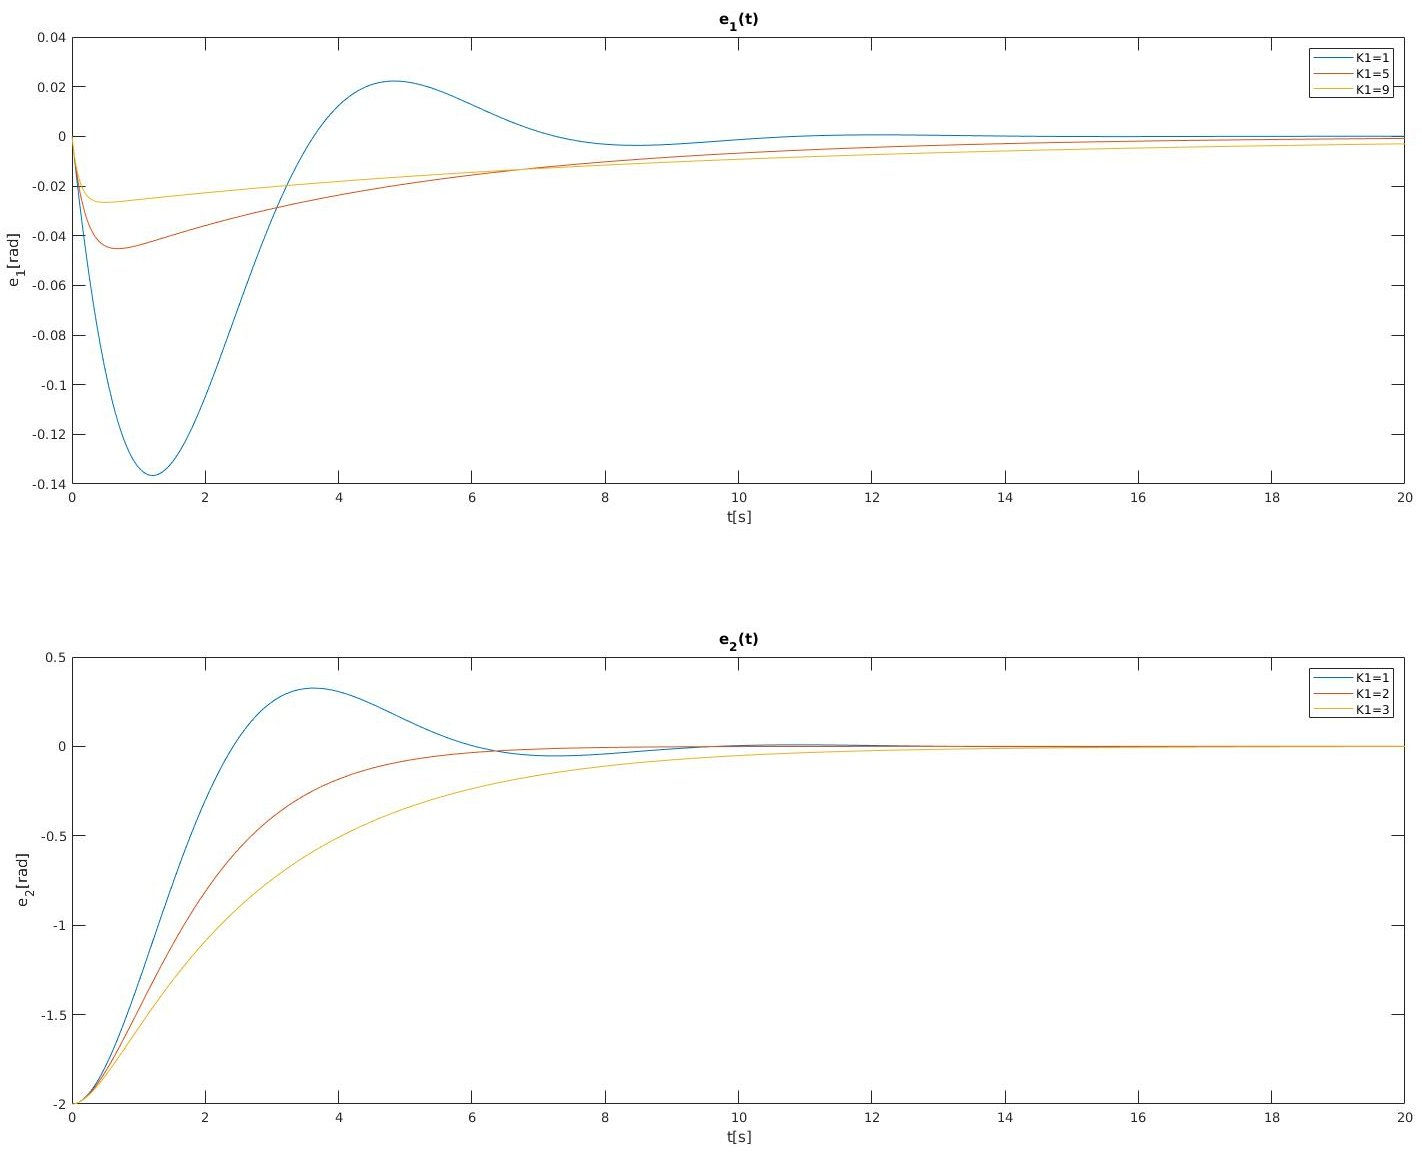
\includegraphics[height=0.50\textheight]{figures/lin2.jpg}
    \caption{stałe KP = 1, zmienne KD}
    \label{fig:lin2}
  \end{figure}



  \subsection{Zależność od wartości początkowej}
  \subsection{Wnioski}

\section{Podsumowanie}


\end{document}